\documentclass{scrartcl}
\usepackage[a4paper,left=1in,right=1in,top=1.2in,bottom=1in]{geometry}
\usepackage{siunitx}
\usepackage{graphicx}
\setkomafont{disposition}{\normalfont\bfseries}

%title
\title{Exercise 02:\\Single-compartment model}
\subtitle{Theoretical Neuroscience I}
\author{Maria del Cerro \and Johannes G\"atjen \and Lorena Morton}
%use these for structure/overview
\newcommand\Question{%
  \textbf{Question:}%
}
\newcommand\Answer{%
  \textbf{Answer:}%
}

\begin{document}
\maketitle
\Question\\
Compute and plot the dependent variables of a neuron with the single-compartment model for a constant input current, an oscillating input current with low frequency (10\si{Hz}), an oscillating input current with medium frequency (100\si{Hz}) and a high frequency random input current. Use the following values for the independent variables: $r_m = 0.9\si{\mega\ohm\square\milli\meter}$, $c_m = 12\si{\nano\farad\per\square\milli\meter}$, $V_0 = 0\si{mV}$ and $i_0 = 25 \si{\nano\ampere\per\square\milli\meter}$.
\\\\
\Answer\\

The input current is defined manually by us. We have four cases: A constant input current (Figure~\ref{constant}), a low frequency input current (Figure~\ref{low}), a medium frequency input current (Figure~\ref{medium}) and a high frequency random input current (Figure~\ref{random}).

The equilibrium potential only differs from the input current by a constant factor and is measured in \si{mV} instead of \si{\nano\ampere\per\square\milli\meter}.

The membrane voltage approaches the equilibrium potential over time, with a speed determined by the membrane resistance and membrane capacitance. If the equilibrium potential does not change, the membrane potential will eventually be equal to it. If the equilibrium potential changes more rapidly the membrane potential cannot follow quickly enough and the maximum amplitude is considerably smaller than the amplitude of the equilibrium potential. This can be seen very well in the case of the medium frequency input current in Figure \ref{medium}. The membrane current is directly proportional to the membrane voltage and thus follows the same patterns.

The capacitor current is the difference between the electrode current and the membrane current and is proportional to the change in membrane voltage over time. So when the membrane voltage is already close to the equilibrium potential and does not change much, the capacitor current is low, whereas if the membrane voltage is far away from the equilibrium potential it changes rapidly and the capacitor current is high. As the membrane potential cannot follow a rapidly changing input current quickly enough most of the input current will go into the capacitor current. As a result the amplitude of the capacitor current is much higher, if the frequency of the input current is higher. This can be seen very well by comparing the capacitor currents in Figures \ref{low} and \ref{medium}


\begin{figure}[h]
\centering
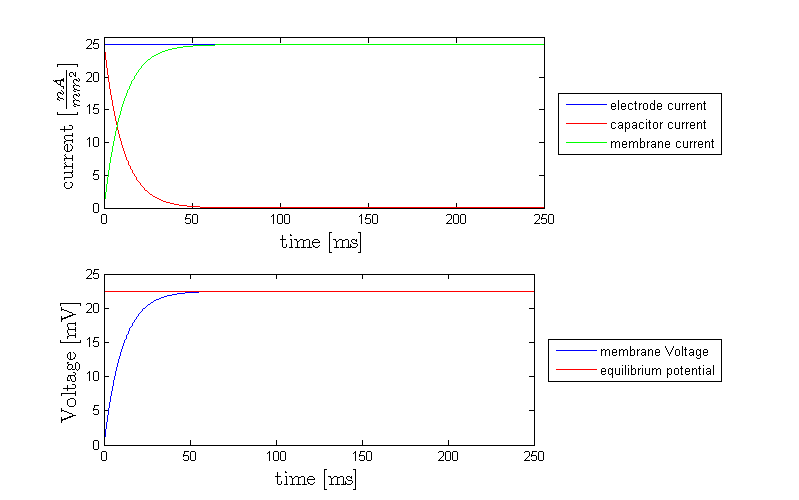
\includegraphics[trim = {1.3cm 0 2cm 0.9cm}, width=\textwidth, clip]{../pics/constant}
\caption{Constant input current: $i_e(t) = i_0$. Top: The electrode current($i_e$, blue), the capacitor current($i_c$, red) and the membrane current ($i_r$, green) over time. Bottom: The membrane voltage ($V_m$, blue) and the equilibrium potential ($V_\infty$, red) over time.}
\label{constant}
\end{figure}


\begin{figure}
\centering
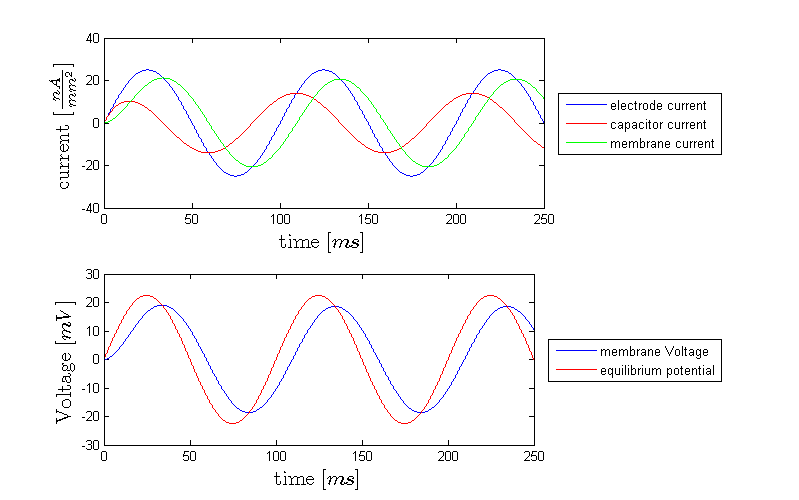
\includegraphics[trim = {1.3cm 0 2cm 0.9cm}, width=\textwidth, clip]{../pics/low}
\caption{Low frequency input current: $i_e(t) = i_0 \cdot \sin{2\pi f t}$ , $f = 10\si{\hertz}$. Same variables shown as in Figure \ref{constant}.}
\label{low}
\end{figure}

\begin{figure}
\centering
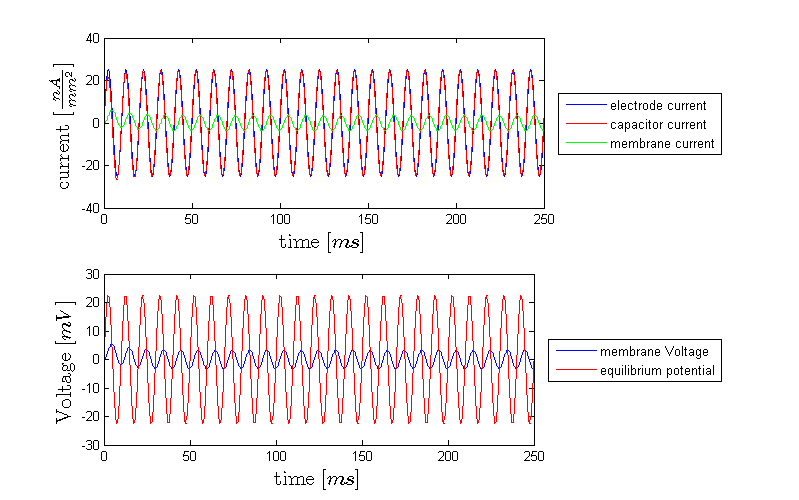
\includegraphics[trim = {1.3cm 0 2cm 0.9cm}, width=\textwidth, clip]{../pics/medium}
\caption{Medium frequency input current: $i_e(t) = i_0 \cdot \sin{2\pi f t}$ , $f = 100\si{\hertz}$. Same variables shown as in Figure \ref{constant}.}
\label{medium}
\end{figure}

\begin{figure}
\centering
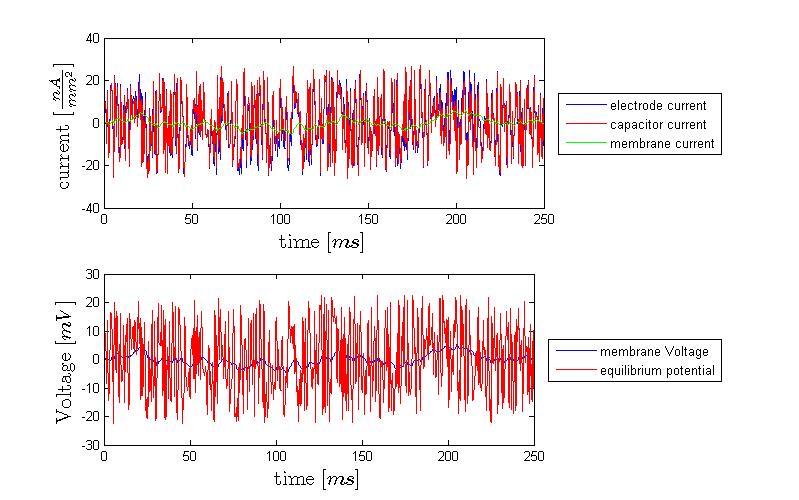
\includegraphics[trim = {1.3cm 0 2cm 0.9cm}, width=\textwidth, clip]{../pics/random}
\caption{High frequency random input current. Same variables shown as in Figure \ref{constant}.}
\label{random}
\end{figure}


\end{document}